\documentclass[aspectratio=169]{beamer}

\usepackage{amsmath, amssymb, amsxtra, amsthm, amsfonts}
\usetheme{moloch}
\usecolortheme{beaver}
\setbeamertemplate{footline}
{
  \leavevmode%
  \hbox{%
    \begin{beamercolorbox}[wd=.5\paperwidth,ht=2.25ex,dp=1ex,center]{author in head/foot}%
      \usebeamerfont{author in head/foot}\insertsection
    \end{beamercolorbox}%
    \begin{beamercolorbox}[wd=.5\paperwidth,ht=2.25ex,dp=1ex,right]{date in head/foot}%
      \usebeamerfont{date in head/foot}\inserttitle\hspace*{2em}
      \insertframenumber{} / \inserttotalframenumber\hspace*{2ex}
    \end{beamercolorbox}}%
  \vskip0pt%
}
\makeatother

\usepackage[english]{babel}
\usefonttheme{serif}

\usepackage{mathtools}
\usepackage{graphicx}
\usepackage{bm}
\usepackage{color}
\usepackage[dvipsnames,table]{xcolor}
\usepackage{tikz}
\usepackage{stanli}
\usepackage{verbatim}
\usepackage{tikz}
\usetikzlibrary{shapes,calc,through,3d,patterns}
\usetikzlibrary{decorations.pathreplacing}
\usetikzlibrary{arrows.meta,calc,positioning}

\usepackage{pgfplots}
\usepackage{siunitx} % For formatting numbers
\usepackage{hyperref}
\hypersetup{colorlinks=true,linkcolor=darkred}
\usepackage{multicol}
\usepackage[absolute,overlay,]{textpos}
\usepackage{pgfplots}
\pgfplotsset{width=10cm,compat=1.9}
\usepackage{subcaption}
\usepackage{multirow}
\usepackage{bbding}
\usepackage{arydshln}
\usepackage{mathtools}
\usepackage{tcolorbox}
\usepackage{animate}

\textblockorigin{80mm}{45mm}


\newtheorem{thm}{Theorem}
\newtheorem{cor}[thm]{Corollary}
\newtheorem{prop}[thm]{Proposition}
\newtheorem{lem}[thm]{Lemma}
\theoremstyle{remark}
\newtheorem*{rem}{Remark}

%Block def
\definecolor{darkred}{rgb}{0.6,0,0}
\setbeamertemplate{blocks}[rounded][shadow=false]
\setbeamercolor{block title}{bg=darkred!15,fg=black}
\setbeamercolor{block body}{bg=darkred!5,fg=black}

\setbeamercolor{itemize item}{fg=darkred}
\setbeamercolor{itemize subitem}{fg=darkred}
\setbeamercolor{itemize subsubitem}{fg=darkred}
\setbeamercolor{enumerate item}{fg=darkred}
\setbeamercolor{button}{bg=gray!30,fg=darkred}

\setbeamertemplate{itemize item}[square]
\setbeamertemplate{itemize subitem}[circle]
\setbeamertemplate{itemize subsubitem}[triangle]
\setbeamertemplate{enumerate items}[circle]
\setbeamercolor{item projected}{bg=darkred}

\newcommand{\bolddelta}{\boldsymbol\delta}
\newcommand{\boldxi}{\boldsymbol\xi}
\DeclareMathOperator*{\A}{\text{\raisebox{-0.2cm}{\Huge A}}}




\title{Dynamic analysis of frames and grids}
\subtitle{Special structural elements}
\author{ME473 Dynamic finite element analysis of structures}
\institute{Stefano Burzio}
\date{2025}

\begin{document}
\usenavigationsymbolstemplate{}
{\setbeamertemplate{footline}{}

  \frame{\titlepage
    \begin{tikzpicture}[overlay, remember picture]
      \node[anchor=north east, xshift=-.9cm] at (current page.north east) {
\includegraphics[width=2cm]{../images/epfl_logo.png}};
      \node[anchor=south east, xshift=-.87cm, yshift=.05cm] at (current page.south east)  {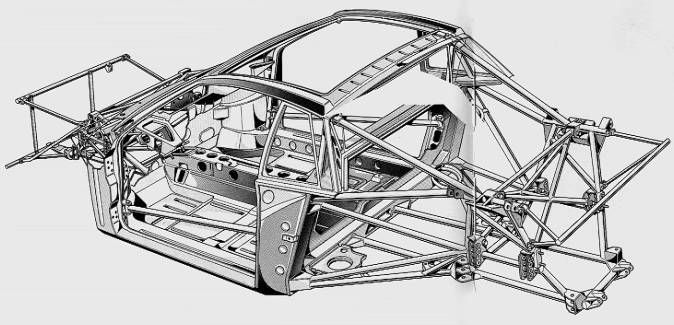
\includegraphics[height=3cm]{../images/tubularChassis.jpg}};
    \end{tikzpicture}
  }

  \begin{frame}{Where do we stand?}
    \begin{center}
      \begin{tabular}{|c|l|l|l|}
        \hline
        \rowcolor{darkred!20}\textbf{Week} & \textbf{Module}                                & \textbf{Lecture topic}             & \textbf{Mini-projects} \\
        \hline

        1                                  & \multirow{5}{7em}{Linear elastodynamics}       & Strong and weak forms              &                        \\ \cline{1-1} \cline{3-4}
        2                                  &                                                & Galerkin method                    &                        \\ \cline{1-1} \cline{3-4}
        3                                  &                                                & Finite element method              & Groups formation       \\ \cline{1-1} \cline{3-4}
        4                                  &                                                & Systematization of the procedure   & Project 1 statement    \\
        \cline{1-1} \cline{3-4}
        5                                  &                                                & 3d elements, numerical integration &                        \\
        \hline
        6                                  & \multirow{3}{7em}{Special structural elements} & Bars and trusses                   &                        \\
        \cline{1-1} \cline{3-4} 7          &                                                & Planar beams                       & Project 1 submission   \\
        \cline{1-1} \cline{3-4} 8          &                                                & Frames and grids                   & Project 2 statement    \\
        \hline
      \end{tabular}
    \end{center}
    \vspace{1cm}
  \end{frame}

  \begin{frame}
    \textbf{\large Summary}
    \begin{itemize}
      \item Recap week 7
      \item Plane frames
      \item Plane grids
      \item Three-dimensional frames
    \end{itemize}
    \vspace{.5cm}

    \textbf{\large Recommended readings}
    \begin{enumerate}
      \item Logan, A first course in the finite element method, 6th ed.
            (chap. 5)
      \item Paz and Leigh, Structural dynamics, 6th ed. (chap. 11, 12 and 13)
      \item Ferreira and Fantuzzi, MATLAB Codes for Finite Element Analysis, 2nd ed. (chap. 7, 8 and 9)
    \end{enumerate}
  \end{frame}
}

\section{Recap week 7 \\ Vibrations of planar beams}
 {\setbeamercolor{background canvas}{bg=darkred!5}
  \setbeamercolor{block body}{bg=darkred!5,fg=black}

  \begin{frame}{Planar thin beam element}
    \vspace{-0.5cm}
    \begin{columns}
      \column{0.5\textwidth}
      \begin{center}
        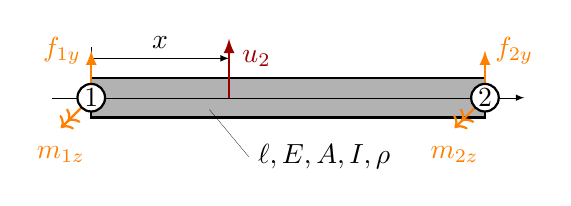
\begin{tikzpicture}[scale=0.5]
          % Draw the rectangle
          \filldraw[fill=gray!60, draw=black,thick] (0,-0.5) rectangle (10,0.5);
          % length
          \draw[ultra thin] (3.5,0) -- (3.5, 1.3) ;
          \draw[ultra thin] (0,0) -- (0, 1.3) ;
          \draw[-latex, ultra thin]  (0,1)  to node[sloped,midway,above] {$x$}(3.5,1) ;
          \draw[ultra thin]  (3,-0.3) -- (4,-1.5) node[right]{$\ell,E,A,I,\rho$};
          %forces
          \draw[thick,-latex,orange] (0,0) -- (0,1.2) node[left]{$f_{1y}$};
          \draw[thick,-latex,orange] (10,0) -- (10,1.2) node[right]{$f_{2y}$};
          % moments 
          \draw[thick,->>,orange] (0,0) -- (0,0,2) node[below=3pt]{$m_{1z}$};
          \draw[thick,->>,orange] (10,0) -- (10,0,2) node[below=3pt]{$m_{2z}$};
          %axis
          \draw[-latex, ultra thin] (-1,0) -- (11,0);
          % Mark points
          \fill (0,0) circle (4pt);
          \fill (10,0) circle (4pt);
          \draw[thick,fill=white] (0,0) circle(0.35cm) node {1};
          \draw[thick,fill=white] (10,0)  circle(0.35cm) node {2};
          % displacement
          \draw[thick,-latex,darkred] (3.5,0) -- (3.5,1.5);
          \node[darkred] at (4.2,1) {$u_2$};
        \end{tikzpicture}
      \end{center}

      \column{0.55\textwidth}
      \vspace{0.3cm}
      \begin{tcolorbox}[colback=darkred!10,colframe=darkred!40!black]
        \small Equation governing the dynamics:
        $$\partial_{x x}^2\big(EI\partial_{x x}^2u_{2}(x,t)\big)+\rho A\ddot u_{2}(x,t)=0$$
      \end{tcolorbox}
    \end{columns}
    \vspace{0.3cm}

    \begin{itemize}
      \item Displacement approximation:
            $$u^h_2(x,t)=  \mathbf H(x)\mathbf q_{loc} (t)=\begin{bmatrix}  h_1(x) & h_2(x) & h_3(x)& h_4(x)\end{bmatrix}\begin{bmatrix}
                q_{1y}(t) \\[2pt] \phi_{1z}(t)\\[2pt] q_{2y}(t)\\[2pt] \phi_{2z}(t)
              \end{bmatrix}$$
      \item Hermite local shape functions:
            \begin{align*}
              h_1(x) & =2(x/\ell)^3-3(x/\ell)^2+1 & h_3(x) & =3(x/\ell)^2-2(x/\ell)^3 \\
              h_2(x) & =x(1-x/\ell)^2             & h_4(x) & =x(x/\ell)(x/\ell-1)     \\
            \end{align*}
    \end{itemize}
  \end{frame}

  \begin{frame}{Discretization of thin beams}
    \begin{itemize}
      \item Element stiffness matrix in local coordinates:
            $$ \small \mathbf{K}_{loc}=\int_0^{\ell} EI\ \frac{d^2\mathbf{H}}{dx^2}^T\frac{d^2\mathbf{H}}{dx^2}\ dx =\frac{EI}{\ell^3} \begin{bmatrix} 12 & 6\ell & -12 & 6\ell \\  & 4\ell^2 & -6\ell & 2\ell^2\\ & &12 & -6\ell \\ sym. & & & 4\ell^2 \end{bmatrix}
            $$
      \item Element consistent mass matrix in local coordinates:
            $$ \small \mathbf{M}_{loc}  =\int_0^{\ell}  \rho A\ \mathbf{H}^T\mathbf{H}\ dx =\frac{\rho A\ell }{420}\begin{bmatrix}
                156  & 22\ell  & 54     & -13\ell  \\
                     & 4\ell^2 & 13\ell & -3\ell^2 \\
                     &         & 156    & -22\ell  \\
                sym. &         &        & 4\ell^2  \\
              \end{bmatrix}
            $$

      \item Element applied loads vector in local coordinates:
            \[ \small \mathbf{f}_{loc}(t) = \begin{bmatrix} f_{1y}(t) \\ m_{1z}(t) \\f_{2y}(t) \\ m_{2z}(t) \end{bmatrix} \]
    \end{itemize}
  \end{frame}

  \begin{frame}{Planar thick beam element}
    \vspace{-0.3cm}
    \begin{columns}
      \column{0.5\textwidth}
      \begin{center}
        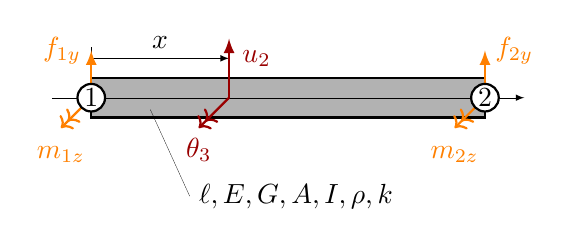
\begin{tikzpicture}[scale=0.5]
          % Draw the rectangle
          \filldraw[fill=gray!60, draw=black,thick] (0,-0.5) rectangle (10,0.5);
          % length
          \draw[ultra thin] (3.5,0) -- (3.5, 1.3) ;
          \draw[ultra thin] (0,0) -- (0, 1.3) ;
          \draw[-latex, ultra thin]  (0,1)  to node[sloped,midway,above] {$x$}(3.5,1) ;
          \draw[ultra thin]  (1.5,-0.3) -- (2.5,-2.5) node[right]{$\ell,E,G,A,I,\rho,k$};
          %forces
          \draw[thick,-latex,orange] (0,0) -- (0,1.2) node[left]{$f_{1y}$};
          \draw[thick,-latex,orange] (10,0) -- (10,1.2) node[right]{$f_{2y}$};
          % moments 
          \draw[thick,->>,orange] (0,0) -- (0,0,2) node[below=3pt]{$m_{1z}$};
          \draw[thick,->>,orange] (10,0) -- (10,0,2) node[below=3pt]{$m_{2z}$};
          %axis
          \draw[-latex, ultra thin] (-1,0) -- (11,0);
          % Mark points
          \fill (0,0) circle (4pt);
          \fill (10,0) circle (4pt);
          \draw[thick,fill=white] (0,0) circle(0.35cm) node {1};
          \draw[thick,fill=white] (10,0)  circle(0.35cm) node {2};
          % displacement
          \draw[thick,-latex,darkred] (3.5,0) -- (3.5,1.5);
          \node[darkred] at (4.2,1) {$u_2$};
          \draw[thick,->>,darkred] (3.5,0) -- (3.5,0,2) node[below]{$\theta_{3}$};
        \end{tikzpicture}
      \end{center}

      \column{0.55\textwidth}
      \vspace{-0.3cm}
      \begin{tcolorbox}[colback=darkred!10,colframe=darkred!40!black]
        \small Equations governing the dynamics:
        \vspace{-0.1cm}
        \begin{align*}
          \partial_{x}\big(kGA(\partial_{x}u_{2}-\theta_{3})\big)+p                        & =\rho A\ddot u_{2}      \\
          \partial_{x}\big(EI\partial_{x}\theta_{3}\big)+kGA(\partial_{x}u_{2}-\theta_{3}) & =\rho I\ddot \theta_{3}
        \end{align*}
      \end{tcolorbox}
    \end{columns}
    \vspace{0.2cm}
    \begin{itemize}
      \item Displacement approximation $\mathbf u^{h}(\mathbf x,t) = \mathbf H(\mathbf x)\mathbf q(t)$:
            $$\begin{bmatrix}
                u_{2}^h(t,x) \\ \theta_{3}^h(t,x)\end{bmatrix}=\begin{bmatrix} h^c_1 & h^c_2(x) & h^c_3(x) & h^c_4(x) \\[0.5em]
                0     & h^l_1(x) & 0        & h^l_2(x)\end{bmatrix}\begin{bmatrix}
                q_{1y}^\prime(t) \\[2pt] \phi_{1z}^\prime(t)\\[2pt] q_{2y}^\prime(t)\\[2pt] \phi_{2z}^\prime(t)
              \end{bmatrix}$$
      \item $h^c_i$ \textbf{Cubic Hermite shape functions} $h^c_i$  are used to approximate the transversal displacement while \textbf{linear shape functions} $h^l_j$ for the rotation.
    \end{itemize}
  \end{frame}

  \begin{frame}{Discretization of thick beams}
    \begin{itemize}
      \item $\mathbf B=\nabla_u\mathbf H$ is the deformation matrix:
            \begin{align*}
              \mathbf B
              =\left[
                \begin{array}{cccc}
                  \partial_x{h_1^c} & \partial_x{h_2^c}-h_1^l & \partial_x{h_3^c} & \partial_x{h_4^c}-h_2^l \\
                  0                 & \partial_x{h_1^l}       & 0                 & \partial_x{h_2^l}
                \end{array}\right]
            \end{align*}
      \item The stiffness $\mathbf K$ and mass $\mathbf{Ma}$ matrices and load vector $\mathbf r$ are defined as
            \begin{align*}
              \mathbf K     =\int_0^\ell \mathbf B^T\mathbf C\mathbf B \, dx,\qquad
              \mathbf{Ma}  =\int_0^\ell \mathbf H^T\mathbf M\mathbf H \, dx,\qquad
              \mathbf r(t)  = \int_{0}^{\ell} \mathbf H^{T}\mathbf f\, dx + \mathbf H^{T}(\ell)\mathbf{\hat f}.
            \end{align*}
      \item Material constitutive matrices:
            $$\mathbf C = \begin{bmatrix}
                kGA & 0  \\
                0   & EI
              \end{bmatrix}\qquad\text{and}\qquad \mathbf M=     \begin{bmatrix}      \rho A & 0      \\
                     0      & \rho I
              \end{bmatrix}$$
    \end{itemize}
  \end{frame}
 }

\section{Plane frames}

\begin{frame}{What is a plane frame?}
  \begin{itemize}
    \item Structure composed of oriented thin beam elements, connected by welding, and carrying \textbf{transversal and axial forces} that all lies in a common plane.
    \item Both forces and moments can be transmitted between members.
    \item Loads are acting only in the common plane of the structure and they must be applied at the joints.
  \end{itemize}\vspace{0.3cm}
  \begin{center}
    \begin{columns}
      \begin{column}{0.48\textwidth}
        \centering
        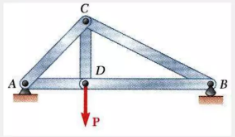
\includegraphics[height=2.3cm]{../images/truss}
        \newline
        \textbf{Plane truss}
      \end{column}

      \begin{column}{0.48\textwidth}
        \centering
        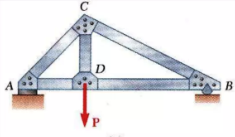
\includegraphics[height=2.3cm]{../images/truss1}
        \newline
        \textbf{Plane frame}
      \end{column}
    \end{columns}
  \end{center}
  \begin{tcolorbox}[colback=darkred!10,colframe=darkred!40!black]
    \centering  \textbf{Truss + Thin beams = Frame}
  \end{tcolorbox}
\end{frame}

{\setbeamercolor{background canvas}{bg=darkred}
\setbeamercolor{block body}{bg=darkred,fg=white}
\setbeamercolor{itemize item}{fg=white}
\setbeamercolor{itemize/enumerate body}{fg=white}
\color{white}
\begin{frame}{Axial loads in thin beam element}
  The inclusion of axial forces in a flexural beam element requires a \emph{superposition} of bar and beam elements:
  \begin{center}
    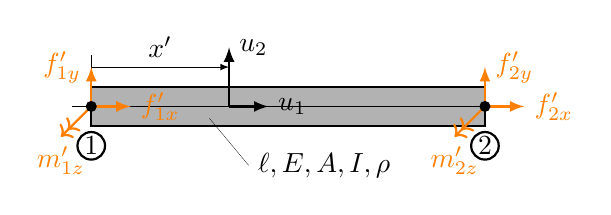
\begin{tikzpicture}[scale=0.5]
      % Draw the rectangle
      \filldraw[fill=gray!60, draw=black,thick] (0,-0.5) rectangle (10,0.5);
      %axis
      \draw[ultra thin] (-0.5,0) -- (10,0);
      % displacement
      \draw[thick,-latex] (3.5,0) -- (3.5,1.5) node[right] {$u_2$};
      \draw[thick,-latex] (3.5,0) -- (4.5,0);
      \node[right] at (4.5,0) {$u_1$};
      % length
      \draw[ultra thin] (3.5,0) -- (3.5, 1.3) ;
      \draw[ultra thin] (0,0) -- (0, 1.3) ;
      \draw[-latex, ultra thin]  (0,1)  to node[sloped,midway,above] {$x^\prime$}(3.5,1) ;
      \draw[ultra thin]  (3,-0.3) -- (4,-1.5) node[right]{$\ell,E,A,I,\rho$}; %forces
      \draw[thick,-latex,orange] (0,0) -- (0,1) node[left]{$f_{1y}^\prime$};
      \draw[thick,-latex,orange] (10,0) -- (10,1) node[right]{$f_{2y}^\prime$};
      \draw[thick,-latex,orange] (0,0) -- (1,0) node[right]{$f_{1x}^\prime$};
      \draw[thick,-latex,orange] (10,0) -- (11,0) node[right]{$f_{2x}^\prime$};
      % moments  
      \draw[thick,->>,orange] (0,0) -- (0,0,2) node[below]{$m_{1z}^\prime$};
      \draw[thick,->>,orange] (10,0) -- (10,0,2) node[below]{$m_{2z}^\prime$};
      % Mark points
      \fill (0,0) circle (4pt);
      \fill (10,0) circle (4pt);
      \draw[thick] (0,0) ++ (0,-1) circle(0.35cm) node {1};
      \draw[thick] (10,0) ++ (0,-1)  circle(0.35cm) node {2};
    \end{tikzpicture}
  \end{center}
  \begin{tcolorbox}[colback=darkred!10,colframe=darkred!40!black]
    Differential equations governing the dynamics:
    \vspace{-0.2cm}
    \begin{align*}
       & \partial_{x^\prime x^\prime}^2\big(EI\partial_{x^\prime x^\prime}^2u_{2}(x^\prime,t)\big)+\rho A\ddot u_{2}(x^\prime,t)=0 \\
       & EA \partial^{2}_{x^\prime x^\prime}u_1(x^\prime, t) = \rho A \ddot{u}_1(x^\prime, t)
    \end{align*}
  \end{tcolorbox}
  \emph{Axial effects are subsequently incorporated into the beam element formulation, unless specified otherwise.
  }
\end{frame}
}

\begin{frame}{Axial displacement in thin beam element}
  A beam element now has three degrees of freedom per node: $q_{ix}^\prime,\  q_{iy}^\prime,$ and $\phi_{iz}^\prime$.

  \begin{itemize}
    \item Displacements approximation:
          $$u^h(x^\prime,t)=  \mathbf H(x^\prime)\mathbf q_{loc} (t)=[{\color{brown}h_1(x^\prime)}\ h_2(x^\prime)\  h_3(x^\prime)\ {\color{brown}h_4(x^\prime)}\  h_5(x^\prime)\ h_6(x^\prime)]\begin{bmatrix}
              {\color{brown} q_{1x}^\prime(t)} \\[2pt] q_{1y}^\prime(t) \\[2pt] \phi_{1z}^\prime(t)\\[2pt]  {\color{brown} q_{2x}^\prime(t)}\\[2pt]  q_{2y}^\prime(t)\\[2pt] \phi_{2z}^\prime(t)
            \end{bmatrix}$$
    \item Local shape functions:
          \begin{align*}
            {\color{brown}h_1(x^\prime)} & = {\color{brown}1-x^\prime/\ell}         & {\color{brown}h_4(x^\prime)} & {\color{brown}=x^\prime/\ell}             \\
            h_2(x^\prime)                & =2(x^\prime/\ell)^3-3(x^\prime/\ell)^2+1 & h_5(x^\prime)                & =3(x^\prime/\ell)^2-2(x^\prime/\ell)^3    \\
            h_3(x^\prime)                & =x^\prime(1-x^\prime/\ell)^2             & h_6(x^\prime)                & =x^\prime(x^\prime/\ell)(x^\prime/\ell-1) \\
          \end{align*}
  \end{itemize}
\end{frame}


\begin{frame}{Discretization of thin beam including axial effects}
  \begin{itemize}
    \item Element stiffness matrix in local coordinates:
          $$\small \mathbf{K}_{loc}=\frac{EI}{\ell^3} \begin{bmatrix}
              {\color{brown}A\ell^2/I} & 0  & 0       & {\color{brown}-A\ell^2/I} & 0      & 0       \\
                                       & 12 & 6\ell   & 0                         & -12    & 6\ell   \\
                                       &    & 4\ell^2 & 0                         & -6\ell & 2\ell^2 \\
                                       &    &         & {\color{brown}A\ell^2/I}  & 0      & 0       \\
                                       &    &         &                           & 12     & -6\ell  \\ sym. & & & & & 4\ell^2\end{bmatrix}
          $$
    \item Element consistent mass matrix in local coordinates:
          \[\small  \mathbf{M}_{loc} =\frac{\rho A\ell }{420}\begin{bmatrix}
              {\color{brown}140} & 0   & 0       & {\color{brown}70} & 0      & 0        \\
              0                  & 156 & 22\ell  & 0                 & 54     & -13\ell  \\
                                 &     & 4\ell^2 & 0                 & 13\ell & -3\ell^2 \\
                                 &     &         & {\color{brown}70} & 0      & 0        \\
                                 &     &         &                   & 156    & -22\ell  \\
              sym.               &     &         &                   &        & 4\ell^2  \\
            \end{bmatrix} \]
  \end{itemize}
\end{frame}

\begin{frame}{Arbitrarly oriented thin beam element including axial effects}
  \vspace{-0.4cm}
  \begin{columns}
    \column{0.5\textwidth}
    \begin{itemize}
      \item Displacements in local coordinates:\vspace{-0.3cm}  $$\mathbf{q}_{loc} = \begin{bmatrix}
                q_{1x}^\prime & q_{1y}^\prime & \phi_{1z}^\prime & q_{2x}^\prime & q_{2y}^\prime & \phi_{2z}^\prime
              \end{bmatrix}^T.$$
      \item Displacements in global coordinates:\vspace{-0.3cm} $$\mathbf q =  \begin{bmatrix}
                q_{1x} & q_{1y} & \phi_{1z} & q_{2x} & q_{2y} & \phi_{2z}
              \end{bmatrix}^T.$$
      \item       \textbf{Relation between local and global displacements:}
    \end{itemize}
    \column{0.5\textwidth}
    \begin{center}
      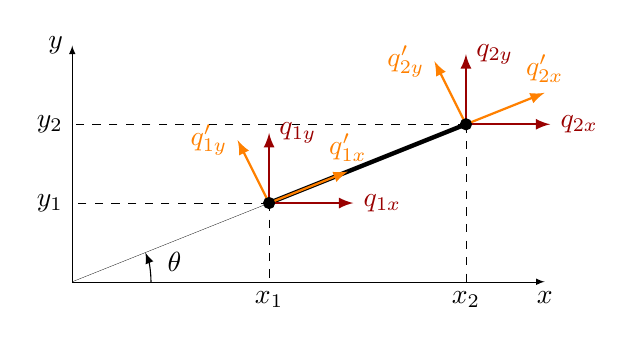
\begin{tikzpicture}[scale=1]
        % Draw background grid
        %\draw[step=1cm,gray,very thin] (0,0) grid (12,6);
        % Define coordinates
        \coordinate (A) at (0,0);
        \coordinate (B) at (2.5,1);
        \coordinate (C) at (5,2);
        % Draw the truss members
        \draw[ultra thin] (A) -- (B);
        \draw[ultra thick] (B) -- (C);
        % Global coordinate system
        \draw[-latex, ultra thin] (0,0) -- (0,3) node[left] {$y$};
        \draw[-latex, ultra thin] (0,0) -- (6,0) node[below] {$x$};
        % Local coordinate systems
        \draw[-latex, darkred,thick] (B) -- ++(1.07,0) node[right] {$q_{1x}$};
        \draw[-latex, darkred,thick] (C) -- ++(1.07,0) node[right] {$q_{2x}$};
        \draw[-latex, darkred,thick] (B) -- ++(0,0.89) node[right] {$q_{1y}$};
        \draw[-latex, darkred,thick] (C) -- ++(0,0.89) node[right] {$q_{2y}$};
        % Local primed coordinate system
        \draw[-latex, orange, thick] (B) -- ++(1,0.4) node[above] {$q_{1x}^\prime$};
        \draw[-latex, orange, thick] (C) -- ++(1,0.4) node[above] {$q_{2x}^\prime$};
        \draw[-latex, orange, thick] (B) -- ++(-0.4,0.8) node[left] {$q_{1y}^\prime$};
        \draw[-latex, orange, thick] (C) -- ++(-0.4,0.8) node[left] {$q_{2y}^\prime$};
        % Angles and labels
        \draw[-latex] (1,0) arc (0:21.8:1);
        \node at (1.3,0.25) {$\theta$};
        % Draw supports (circles at joints)
        \filldraw (B) circle (2pt);
        \filldraw (C) circle (2pt);
        % Nodes coord
        \draw[dashed,ultra thin] (B) -- (2.5,0) node[below] {$x_1$};
        \draw[dashed,ultra thin] (B) -- (0,1) node[left] {$y_1$};
        \draw[dashed,ultra thin] (C) -- (5,0) node[below] {$x_2$};
        \draw[dashed,ultra thin] (C) -- (0,2) node[left] {$y_2$};
      \end{tikzpicture}
    \end{center}
  \end{columns}
  $$\small \underbrace{\begin{bmatrix}
        q_{1x}^\prime \\ q_{1y}^\prime \\ \phi_{1z}^\prime \\  q_{2x}^\prime\\ q_{2y}^\prime \\ \phi_{2z}^\prime
      \end{bmatrix}}_\text{$\mathbf q_{loc}$}=\underbrace{\begin{bmatrix}
        \cos(\theta)  & \sin(\theta) & 0 & 0             & 0            & 0 \\
        -\sin(\theta) & \cos(\theta) & 0 & 0             & 0            & 0 \\
        0             & 0            & 1 & 0             & 0            & 0 \\
        0             & 0            & 0 & \cos(\theta)  & \sin(\theta) & 0 \\
        0             & 0            & 0 & -\sin(\theta) & \cos(\theta) & 0 \\
        0             & 0            & 0 & 0             & 0            & 1 \\
      \end{bmatrix}}_\text{$\mathbf T$}\underbrace{\begin{bmatrix}
        q_{1x} \\ q_{1y} \\ \phi_{1z} \\ q_{2x} \\ q_{2y} \\ \phi_{2z}
      \end{bmatrix}}_\text{$\mathbf q$}
  $$
\end{frame}

\begin{frame}{Discretization of arbitrarly oriented beam including axial effects}
  \begin{itemize}
    \item Element stiffness matrix in global coordinates:
          $$\tiny \mathbf{K} = \mathbf T^T \mathbf{K}_{loc} \mathbf T=\frac{E}{\ell}\begin{bmatrix}
              \frac{A \ell^3 C^2 + 12 I S^2}{\ell^2} & \frac{(-12 I + A \ell^2) C S}{\ell^2}  & \frac{-6 I S}{\ell} & -\frac{A \ell^3 C^2 + 12 I S^2}{\ell^2} & \frac{(12 I - A \ell^2) C S}{\ell^2}    & \frac{-6 I S}{\ell} \\
                                                     & \frac{12 I C^2 + A \ell^2 S^2}{\ell^2} & \frac{6 I C}{\ell}  & \frac{(12 I - A \ell^2) C S}{\ell^2}    & -\frac{12 I C^2 + A \ell^2 S^2}{\ell^2} & \frac{6 I C}{\ell}  \\
                                                     &                                        & 4 I                 & \frac{6 I S}{\ell}                      & \frac{-6 I C}{\ell}                     & 2 I                 \\
                                                     &                                        &                     & \frac{A \ell^3 C^2 + 12 I S^2}{\ell^2}  & \frac{(-12 I + A \ell^2) C S}{\ell^2}   & \frac{6 I S}{\ell}  \\
                                                     &                                        &                     &                                         & \frac{12 I C^2 + A \ell^2 S^2}{\ell^2}  & \frac{-6 I C}{\ell} \\
                                                     &                                        &                     &                                         &                                         & 4 I
            \end{bmatrix}$$
          where $C=\cos(\theta)$ and $S=\sin(\theta)$.
          \vspace{0.3cm}
    \item Element consistent mass matrix in global coordinates:
          $$\mathbf{M} = \mathbf T^T \mathbf{M}_{loc} \mathbf T$$
  \end{itemize}
\end{frame}

\begin{frame}{Applied loads}
  \begin{itemize}
    \item Element applied loads vector in local coordinates:
          \[ \small \mathbf{f}_{loc}(t) = \begin{bmatrix} {\color{brown}f_{1x}^\prime(t)} \\ f_{1y}^\prime(t) \\ m_{1z}^\prime(t) \\{\color{brown}f_{2x}^\prime(t)} \\f_{2y}^\prime(t) \\ m_{2z}^\prime(t) \end{bmatrix} \]
    \item Element applied loads vector in global coordinates:
          \[
            \mathbf{f} = \mathbf T^T \mathbf{f}_{loc} =\begin{bmatrix}
              \cos(\theta)f_{1x}^\prime + \sin(\theta)f_{1y}^\prime \\
              -\sin(\theta)f_{1x}^\prime +\cos(\theta)f_{1y}^\prime \\
              m_{1z}^\prime                                         \\
              \cos(\theta)f_{2x}^\prime + \sin(\theta)f_{2y}^\prime \\
              -\sin(\theta)f_{2x}^\prime +\cos(\theta)f_{2y}^\prime \\
              m_{2z}^\prime                                         \\
            \end{bmatrix}
          \]
  \end{itemize}
\end{frame}


{\setbeamercolor{background canvas}{bg=darkred}
\setbeamercolor{block body}{bg=darkred,fg=white}
\setbeamercolor{itemize item}{fg=white}
\setbeamercolor{itemize/enumerate body}{fg=white}
\color{white}
\begin{frame}{Assembly of stiffness and mass matrices and loads vector}
  Given a 2d frame structure made of $m$ oriented beams, $n$ nodes, and $3$ DOFs per node:

  \vspace{0.5em}
  \textbf{1. Element quantities:}
  \begin{itemize}
    \item For each beam $e$, compute the element quantities global coordinates:
          \begin{align*}
            {}^e\mathbf{K} & ={}^e\mathbf{T}^{T} {}^e\mathbf{K}_{loc}{}^e\mathbf{T} \\
            {}^e\mathbf{M} & ={}^e\mathbf{T}^{T} {}^e\mathbf{M}_{loc}{}^e\mathbf{T} \\
            {}^e\mathbf{f} & ={}^e\mathbf{T}^{T} {}^e\mathbf{f}_{loc}
          \end{align*}
  \end{itemize}

  \vspace{0.5em}
  \textbf{2. Global assembly:}
  \begin{itemize}
    \item Initialize global stiffness matrix $\mathbf{K}$ and global mass matrix $\mathbf{M}$ of size $3n \times 3n$,
    \item  Initialize global loads vector $\mathbf{f}$ of size $3n \times 1$,
    \item Assemble each ${}^e\mathbf{K}$, ${}^e\mathbf{M}$ and ${}^e\mathbf{f}$ for $e=1,\dots,m$, into $\mathbf{K}$, $\mathbf{M}$ and $\mathbf{f}$ respectively using element connectivity.
  \end{itemize}
\end{frame}
}

\begin{frame}{MATLAB example - a 2d frame in free vibration}
  \begin{center}
    \href{https://drive.mathworks.com/sharing/6a9792ef-d0a7-4aca-a1d0-8b1862b0ac3b}{\beamergotobutton{Go to Matlab Drive}}
  \end{center}
\end{frame}

\section{Plane grids}
\begin{frame}{What is a grid?}
  \begin{itemize}
    \item A grid is a structure composed of oriented planar beams subjected to \textbf{perpendicular loading} that produced significant bending effects.
    \item Beams are connected by welding: both forces and moments can be transmitted between members.
    \item Axial effect of axial displacement is ignored for the moment.
    \item Common type of structures used in to model floors, roofs, bridge decks, etc..
  \end{itemize}
  \begin{center}
    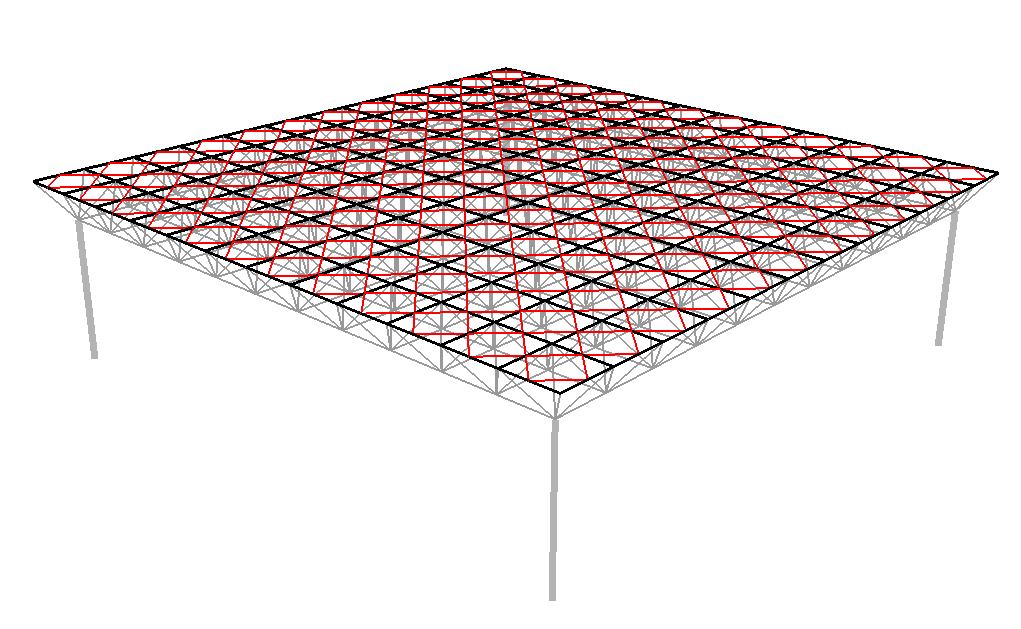
\includegraphics[height=3cm]{../images/grid.png}
  \end{center}
\end{frame}

\begin{frame}{Degrees of freedom identification}
  \vspace{-0.1cm}
  \begin{itemize}
    \item \textbf{Planar frame under action of loads in the plane of the structure:}
          \vspace{-0.1cm}
          \begin{tcolorbox}[colback=darkred!10,colframe=darkred!40!black]
            \small Components required to describe the displacements of joint $i$ are:
            \begin{itemize}
              \item $q_{ix}$ translation in the $x$ direction,
              \item $q_{iy}$ translation in the $y$ direction,
              \item $\phi_{iz}$ bending, rotation about the $z$ axis.
            \end{itemize}
          \end{tcolorbox}
    \item \textbf{Planar grids loaded perpendicularly to the plane of the structure:}
          \vspace{-0.1cm}
          \begin{tcolorbox}[colback=darkred!10,colframe=darkred!40!black]
            \small Components required to describe the displacements of joint $i$ are:
            \begin{itemize}
              \item $q_{iz}$ translation in the $z$ direction,
              \item $\phi_{ix}$  torsion, rotation about the $x$ axis .
              \item $\phi_{iy}$ bending, rotation about the $z$ axis.
            \end{itemize}
          \end{tcolorbox}
  \end{itemize}
\end{frame}

\begin{frame}{Shaft element}
  The development of a shaft finite element is very similar to the development of a bar finite element, where
  \begin{itemize}
    \item the axial displacement $u_1$ is replaced by the angular rotation $\phi_{1}$,
    \item the axial nodal forces $f_{ix}^\prime$ are replaced by nodal torque $m_{ix}^\prime$,
    \item the element tensile stiffness $AE/\ell$ is replaced by the torsional stiffness $GJ/\ell$.
  \end{itemize}
  \begin{columns}
    \column{0.5\textwidth}
    \begin{center}
      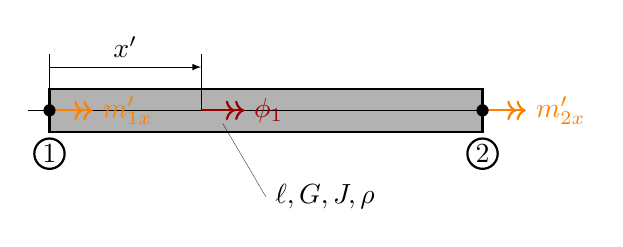
\begin{tikzpicture}[scale=0.55]
        % Draw the rectangle
        \filldraw[fill=gray!60, draw=black,thick] (0,-0.5) rectangle (10,0.5);
        %axis
        \draw[ultra thin] (-0.5,0) -- (10,0);
        %forces
        \draw[thick,->>,orange] (0,0) -- (1,0) node[right]{$m_{1x}^\prime$};
        \draw[thick,->>,orange] (10,0) -- (11,0) node[right]{$m_{2x}^\prime$};
        % Mark points
        \fill (0,0) circle (4pt);
        \fill (10,0) circle (4pt);
        \draw[thick] (0,0) ++ (0,-1) circle(0.35cm) node {1};
        \draw[thick] (10,0) ++ (0,-1)  circle(0.35cm) node {2};
        % displacement
        \draw[thick,->>,darkred] (3.5,0) -- (4.5,0);
        \node[darkred,right] at (4.5,0) {$\phi_{1}$};
        % length
        \draw[ultra thin] (3.5,0) -- (3.5, 1.3) ;
        \draw[ultra thin] (0,0) -- (0, 1.3) ;
        \draw[-latex, ultra thin]  (0,1)  to node[sloped,midway,above] {$x^\prime$}(3.5,1) ;
        \draw[ultra thin]  (4,-0.3) -- (5,-2) node[right]{$\ell,G,J,\rho$};
      \end{tikzpicture}
    \end{center}

    \column{0.4\textwidth}
    {\tiny \begin{itemize}
        \item $G$ shear modulus of the material
        \item $J$ polar moment of inertia of the cross-section.
        \item $\rho$ material density
        \item $\ell$ length
        \item $\phi_{1}$ angular rotation
        \item $x^\prime$ (local) axial coordinate
      \end{itemize}}
  \end{columns}
  \vspace{0.4cm}
\end{frame}


\begin{frame}{Equation of motion for non-oriented shaft element}
  \begin{block}{}
    Differential equation governing the dynamics:
    $$ GJ \partial^{2}_{x^\prime x^\prime}\phi_{1}(x^\prime, t) = \rho J \ddot{\phi}_1(x^\prime, t) $$
  \end{block}

  \begin{itemize}
    \item  Angular rotation (twisting) approximation:
          \[\phi^h_1(x^\prime,t)=  \mathbf H(x^\prime)\mathbf q_{loc} (t)=\begin{bmatrix}  h_1(x^\prime) & h_2(x^\prime)\end{bmatrix} \begin{bmatrix}  \phi_{1x}^\prime(t) \\ \phi_{2x}^\prime(t)\end{bmatrix}\]
    \item Linear local shape functions:
          $$h_1(x^\prime)  =1-\frac{x^\prime}{\ell} \qquad\text{and}\qquad h_2(x^\prime)  =\frac{x^\prime}{\ell}$$
    \item Semi-discrete weak form:
          \[\bolddelta\mathbf{q}_{loc}^T\big(\mathbf{M}_{loc} \ddot{\mathbf{q}}_{loc}(t) + \mathbf{K}_{loc} \mathbf{q}_{loc}(t) - \mathbf{f}_{loc}(t)\big)=0 \]
  \end{itemize}
\end{frame}

\begin{frame}{Discretization of shaft}
  \begin{itemize}
    \item Element stiffness matrix in local coordinates:
          \[ \mathbf{K}_{loc} =\int_0^{\ell}  GJ\ \frac{d\mathbf{H}}{dx^\prime}^T\frac{d\mathbf{H}}{dx^\prime}\ dx^\prime =\int_0^{\ell}  GJ \begin{bmatrix} (h_1^\prime)^2 & h_1^\prime h_2^\prime \\  h_2^\prime h_1^\prime &  (h_2^\prime)^2 \end{bmatrix} dx^\prime =\frac{GJ}{\ell} \begin{bmatrix} 1 & -1 \\ -1 & 1 \end{bmatrix} \]
    \item Element consistent mass matrix in local coordinates:
          \[ \mathbf{M}_{loc} =\int_0^{\ell}  \rho J\ \mathbf{H}^T\mathbf{H}\ dx^\prime =\int_0^{\ell}\rho J \begin{bmatrix} (h_1)^2 &h_1 h_2 \\  h_2 h_1 &  (h_2)^2 \end{bmatrix} dx^\prime =\frac{\rho J\ell }{6} \begin{bmatrix} 2 & 1 \\ 1 & 2 \end{bmatrix} \]
    \item Element applied loads vector in local coordinates:
          \[ \mathbf{f}_{loc}(t) =\begin{bmatrix} h_1(0) \\ h_2(0)\end{bmatrix}m_{1x}^\prime(t) + \begin{bmatrix} h_1(\ell) \\ h_2(\ell)\end{bmatrix}m_{2x}^\prime(t) = \begin{bmatrix} m_{1x}^\prime(t) \\ m_{2x}^\prime(t) \end{bmatrix} \]
  \end{itemize}
\end{frame}


\begin{frame}{}
  \begin{tcolorbox}[colback=darkred!10,colframe=darkred!40!black]
    \centering  \textbf{Shaft + Thin beams = Grid}
  \end{tcolorbox}
  \begin{center}
    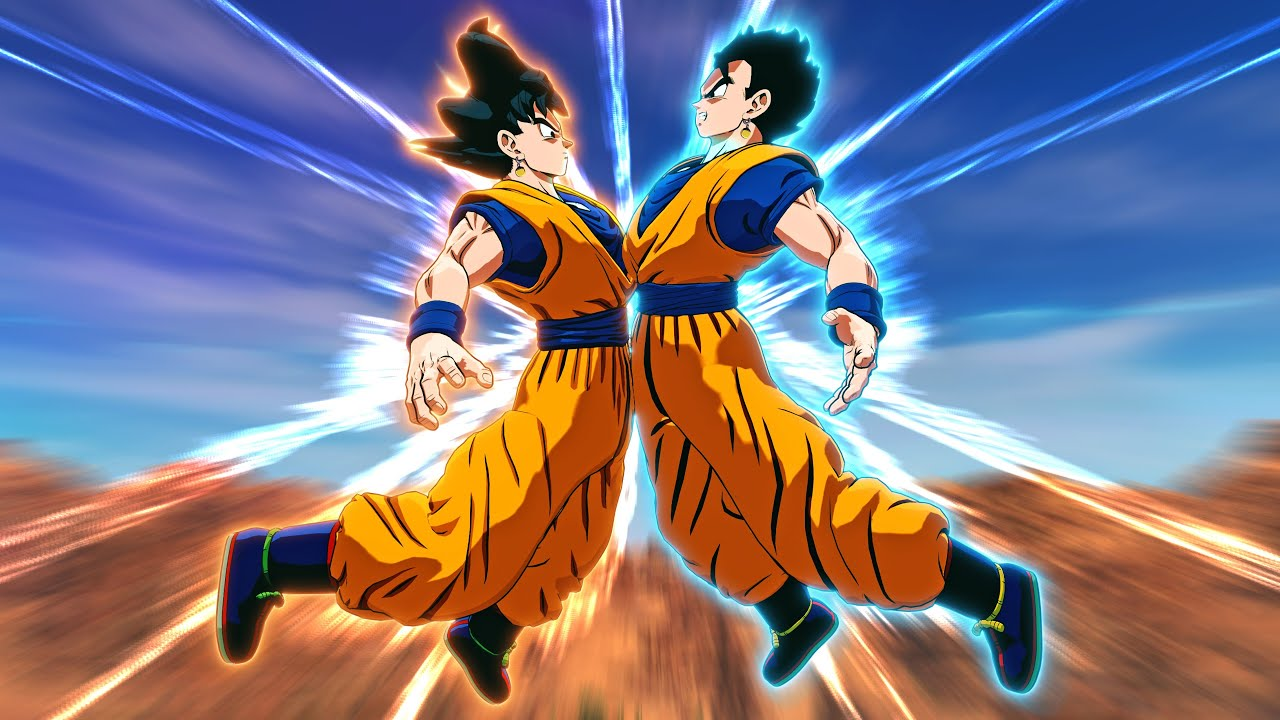
\includegraphics[width=9cm]{../images/fusion1.jpg}
  \end{center}
\end{frame}

{\setbeamercolor{background canvas}{bg=darkred}
\setbeamercolor{block body}{bg=darkred,fg=white}
\setbeamercolor{itemize item}{fg=white}
\setbeamercolor{itemize/enumerate body}{fg=white}
\color{white}
\begin{frame}{Torsional effects in thin beam element}
  The inclusion of torsional stiffness in a thin beam element, to model a typical element in a planar grid frame, requires a \emph{superposition} of shaft and beam elements:
  \begin{center}
    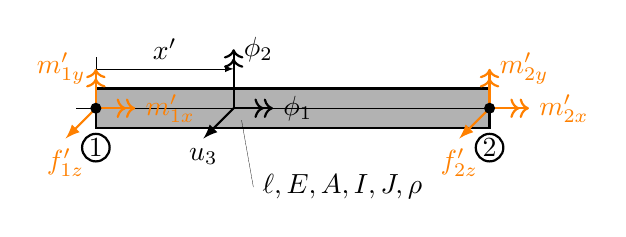
\begin{tikzpicture}[scale=0.5]
      % Draw the rectangle
      \filldraw[fill=gray!60, draw=black,thick] (0,-0.5) rectangle (10,0.5);
      %axis
      \draw[ultra thin] (-0.5,0) -- (10,0);
      % displacement
      \draw[thick,->>] (3.5,0) -- (3.5,1.5) node[right] {$\phi_2$};
      \draw[thick,->>] (3.5,0) -- (4.5,0) node[right] {$\phi_1$};
      \draw[thick,-latex] (3.5,0) -- (3.5,0,2) node[below] {$u_3$};
      % length
      \draw[ultra thin] (3.5,0) -- (3.5, 1.3) ;
      \draw[ultra thin] (0,0) -- (0, 1.3) ;
      \draw[-latex, ultra thin]  (0,1)  to node[sloped,midway,above] {$x^\prime$}(3.5,1) ;
      \draw[ultra thin]  (3.7,-0.3) -- (4,-2) node[right]{$\ell,E,A,I,J,\rho$}; %forces
      \draw[thick,->>,orange] (0,0) -- (0,1) node[left]{$m_{1y}^\prime$};
      \draw[thick,->>,,orange] (10,0) -- (10,1) node[right]{$m_{2y}^\prime$};
      \draw[thick,->>,orange] (0,0) -- (1,0) node[right]{$m_{1x}^\prime$};
      \draw[thick,->>,orange] (10,0) -- (11,0) node[right]{$m_{2x}^\prime$};
      % moments 
      \draw[thick,-latex,orange] (0,0) -- (0,0,2) node[below]{$f_{1z}^\prime$};
      \draw[thick,-latex,orange] (10,0) -- (10,0,2) node[below]{$f_{2z}^\prime$};
      % Mark points
      \fill (0,0) circle (4pt);
      \fill (10,0) circle (4pt);
      \draw[thick] (0,0) ++ (0,-1) circle(0.35cm) node {1};
      \draw[thick] (10,0) ++ (0,-1)  circle(0.35cm) node {2};
    \end{tikzpicture}
  \end{center}
  \begin{tcolorbox}[colback=darkred!10,colframe=darkred!40!black]
    Differential equations governing the dynamics:
    \begin{align*}
       & \partial_{x^\prime x^\prime}^2\big(EI\partial_{x^\prime x^\prime}^2u_{3}(x^\prime,t)\big)+\rho A\ddot u_{3}(x^\prime,t)=0 \\
       & GJ \partial^{2}_{x^\prime x^\prime}\phi_{1}(x^\prime, t) = \rho J \ddot{\phi}_1(x^\prime, t)
    \end{align*}
  \end{tcolorbox}
\end{frame}
}

\begin{frame}{Torsional effects in thin beam element}
  Each grid element now has three degrees of freedom per node: $\phi_{ix}^\prime$, $\phi_{iy}^\prime$ and $q_{iz}^\prime$.

  \begin{itemize}
    \item Displacements approximation:
          $$u^h(x^\prime,t)=  \mathbf H(x^\prime)\mathbf q_{loc} (t)=[{\color{BlueViolet}h_1(x^\prime)}\ h_2(x^\prime)\  h_3(x^\prime)\ {\color{BlueViolet}h_4(x^\prime)}\  h_5(x^\prime)\ h_6(x^\prime)]\begin{bmatrix}
              {\color{BlueViolet} \phi_{1x}^\prime(t)} \\[2pt] \phi_{1y}^\prime(t) \\[2pt] q_{1z}^\prime(t)\\[2pt]  {\color{BlueViolet} \phi_{2x}^\prime(t)}\\[2pt] \phi_{2y}^\prime(t) \\[2pt]  q_{2z}^\prime(t)
            \end{bmatrix}$$
    \item Local shape functions:
          \begin{align*}
            {\color{BlueViolet}h_1(x^\prime)} & = {\color{BlueViolet}1-x^\prime/\ell}    & {\color{BlueViolet}h_4(x^\prime)} & {\color{BlueViolet}=x^\prime/\ell}        \\
            h_2(x^\prime)                     & =x^\prime(1-x^\prime/\ell)^2             & h_5(x^\prime)                     & =x^\prime(x^\prime/\ell)(x^\prime/\ell-1) \\
            h_3(x^\prime)                     & =2(x^\prime/\ell)^3-3(x^\prime/\ell)^2+1 & h_6(x^\prime)                     & =3(x^\prime/\ell)^2-2(x^\prime/\ell)^3    \\
          \end{align*}
  \end{itemize}
\end{frame}


\begin{frame}{Discretization of thin beam with torsional effects}
  \begin{itemize}
    \item Element stiffness matrix in local coordinates:
          $$\small \mathbf{K}_{loc}=\frac{EI}{\ell^3} \begin{bmatrix}
              {\color{BlueViolet}GJ\ell^2/EI} & 0       & 0      & {\color{BlueViolet}-GJ\ell^2/EI} & 0       & 0     \\
                                              & 4\ell^2 & -6\ell & 0                                & 2\ell^2 & 6\ell \\
                                              &         & 12     & 0                                & -6\ell  & -12   \\
                                              &         &        & {\color{BlueViolet}GJ\ell^2/EI}  & 0       & 0     \\
                                              &         &        &                                  & 4\ell^2 & 6\ell \\ sym. & & & & & 12\end{bmatrix}
          $$
    \item Element consistent mass matrix in local coordinates:
          \[\small  \mathbf{M}_{loc} =\frac{\rho A\ell }{420}\begin{bmatrix}
              {\color{BlueViolet}140 J/A} & 0       & 0      & {\color{BlueViolet}70 J/A}  & 0        & 0       \\
              0                           & 4\ell^2 & 22\ell & 0                           & -3\ell^2 & 13\ell  \\
                                          &         & 156    & 0                           & -13\ell  & 54      \\
                                          &         &        & {\color{BlueViolet}140 J/A} & 0        & 0       \\
                                          &         &        &                             & 4\ell^2  & -22\ell \\
              sym.                        &         &        &                             &          & 156     \\
            \end{bmatrix} \]
  \end{itemize}
\end{frame}


\begin{frame}{Arbitrarly oriented thin beam element with torsional effects}
  \vspace{-0.4cm}
  \begin{columns}
    \column{0.5\textwidth}
    \begin{itemize}
      \item Displacements in local coordinates:\vspace{-0.3cm}  $$\mathbf{q}_{loc} = \begin{bmatrix}
                \phi_{1x}^\prime & \phi_{1y}^\prime & q_{1z}^\prime & \phi_{2x}^\prime & \phi_{2y}^\prime & q_{2z}^\prime
              \end{bmatrix}^T.$$
      \item Displacements in global coordinates:\vspace{-0.3cm} $$\mathbf q =  \begin{bmatrix}
                \phi_{1x} & \phi_{1y} & q_{1z} & \phi_{2x} & \phi_{2y} & q_{2z}
              \end{bmatrix}^T.$$
      \item       \textbf{Relation between local and global displacements:}
    \end{itemize}
    \column{0.5\textwidth}
    \begin{center}
      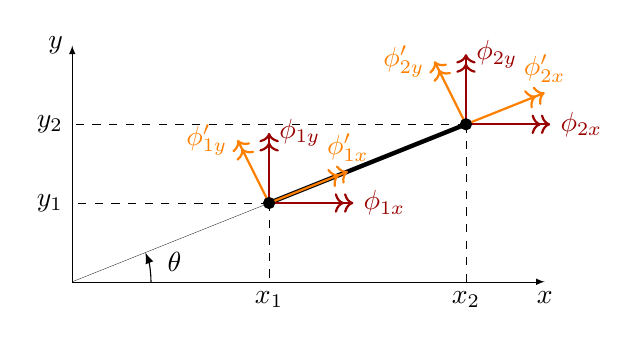
\begin{tikzpicture}[scale=1]
        % Draw background grid
        %\draw[step=1cm,gray,very thin] (0,0) grid (12,6);
        % Define coordinates
        \coordinate (A) at (0,0);
        \coordinate (B) at (2.5,1);
        \coordinate (C) at (5,2);
        % Draw the truss members
        \draw[ultra thin] (A) -- (B);
        \draw[ultra thick] (B) -- (C);
        % Global coordinate system
        \draw[-latex, ultra thin] (0,0) -- (0,3) node[left] {$y$};
        \draw[-latex, ultra thin] (0,0) -- (6,0) node[below] {$x$};
        % Local coordinate systems
        \draw[->>, darkred,thick] (B) -- ++(1.07,0) node[right] {$\phi_{1x}$};
        \draw[->>, darkred,thick] (C) -- ++(1.07,0) node[right] {$\phi_{2x}$};
        \draw[->>, darkred,thick] (B) -- ++(0,0.89) node[right] {$\phi_{1y}$};
        \draw[->>, darkred,thick] (C) -- ++(0,0.89) node[right] {$\phi_{2y}$};
        % Local primed coordinate system
        \draw[->>, orange, thick] (B) -- ++(1,0.4) node[above] {$\phi_{1x}^\prime$};
        \draw[->>, orange, thick] (C) -- ++(1,0.4) node[above] {$\phi_{2x}^\prime$};
        \draw[->>, orange, thick] (B) -- ++(-0.4,0.8) node[left] {$\phi_{1y}^\prime$};
        \draw[->>, orange, thick] (C) -- ++(-0.4,0.8) node[left] {$\phi_{2y}^\prime$};
        % Angles and labels
        \draw[-latex] (1,0) arc (0:21.8:1);
        \node at (1.3,0.25) {$\theta$};
        % Draw supports (circles at joints)
        \filldraw (B) circle (2pt);
        \filldraw (C) circle (2pt);
        % Nodes coord
        \draw[dashed,ultra thin] (B) -- (2.5,0) node[below] {$x_1$};
        \draw[dashed,ultra thin] (B) -- (0,1) node[left] {$y_1$};
        \draw[dashed,ultra thin] (C) -- (5,0) node[below] {$x_2$};
        \draw[dashed,ultra thin] (C) -- (0,2) node[left] {$y_2$};
      \end{tikzpicture}
    \end{center}
  \end{columns}
  $$\small \underbrace{\begin{bmatrix}
        \phi_{1x}^\prime \\ \phi_{1y}^\prime \\ q_{1z}^\prime \\  \phi_{2x}^\prime\\ \phi_{2y}^\prime \\ q_{2z}^\prime
      \end{bmatrix}}_\text{$\mathbf q_{loc}$}=\underbrace{\begin{bmatrix}
        \cos(\theta)  & \sin(\theta) & 0 & 0             & 0            & 0 \\
        -\sin(\theta) & \cos(\theta) & 0 & 0             & 0            & 0 \\
        0             & 0            & 1 & 0             & 0            & 0 \\
        0             & 0            & 0 & \cos(\theta)  & \sin(\theta) & 0 \\
        0             & 0            & 0 & -\sin(\theta) & \cos(\theta) & 0 \\
        0             & 0            & 0 & 0             & 0            & 1 \\
      \end{bmatrix}}_\text{$\mathbf T$}\underbrace{\begin{bmatrix}
        \phi_{1x} \\ \phi_{1y} \\ q_{1z} \\ \phi_{2x} \\ \phi_{2y} \\ q_{2z}
      \end{bmatrix}}_\text{$\mathbf q$}
  $$
\end{frame}

\begin{frame}{Discretization of arbitrarly oriented thin beam}
  \begin{itemize}
    \item Element stiffness matrix in global coordinates:
          $$\mathbf{K} = \mathbf T^T \mathbf{K}_{loc} \mathbf T$$
          where $C=\cos(\theta)$ and $S=\sin(\theta)$.
    \item Element consistent mass matrix in global coordinates:
          $$\mathbf{M} = \mathbf T^T \mathbf{M}_{loc} \mathbf T$$
    \item Element applied loads vector in global coordinates:
          \[
            \mathbf{f} = \mathbf T^T \mathbf{f}_{loc}
          \]
  \end{itemize}
\end{frame}


\begin{frame}{MATLAB example - dynamic response of a 2d grid}
  \begin{center}
    \href{https://drive.mathworks.com/sharing/6a9792ef-d0a7-4aca-a1d0-8b1862b0ac3b}{\beamergotobutton{Go to Matlab Drive}}
  \end{center}
\end{frame}

\section{Three-dimensional frames}

\begin{frame}{Example of a three-dimensional structure composed of thin beams}
  \vspace{-0.5cm}
  \begin{columns}
    \begin{column}{0.35\textwidth}
      \vspace{0.5cm}

      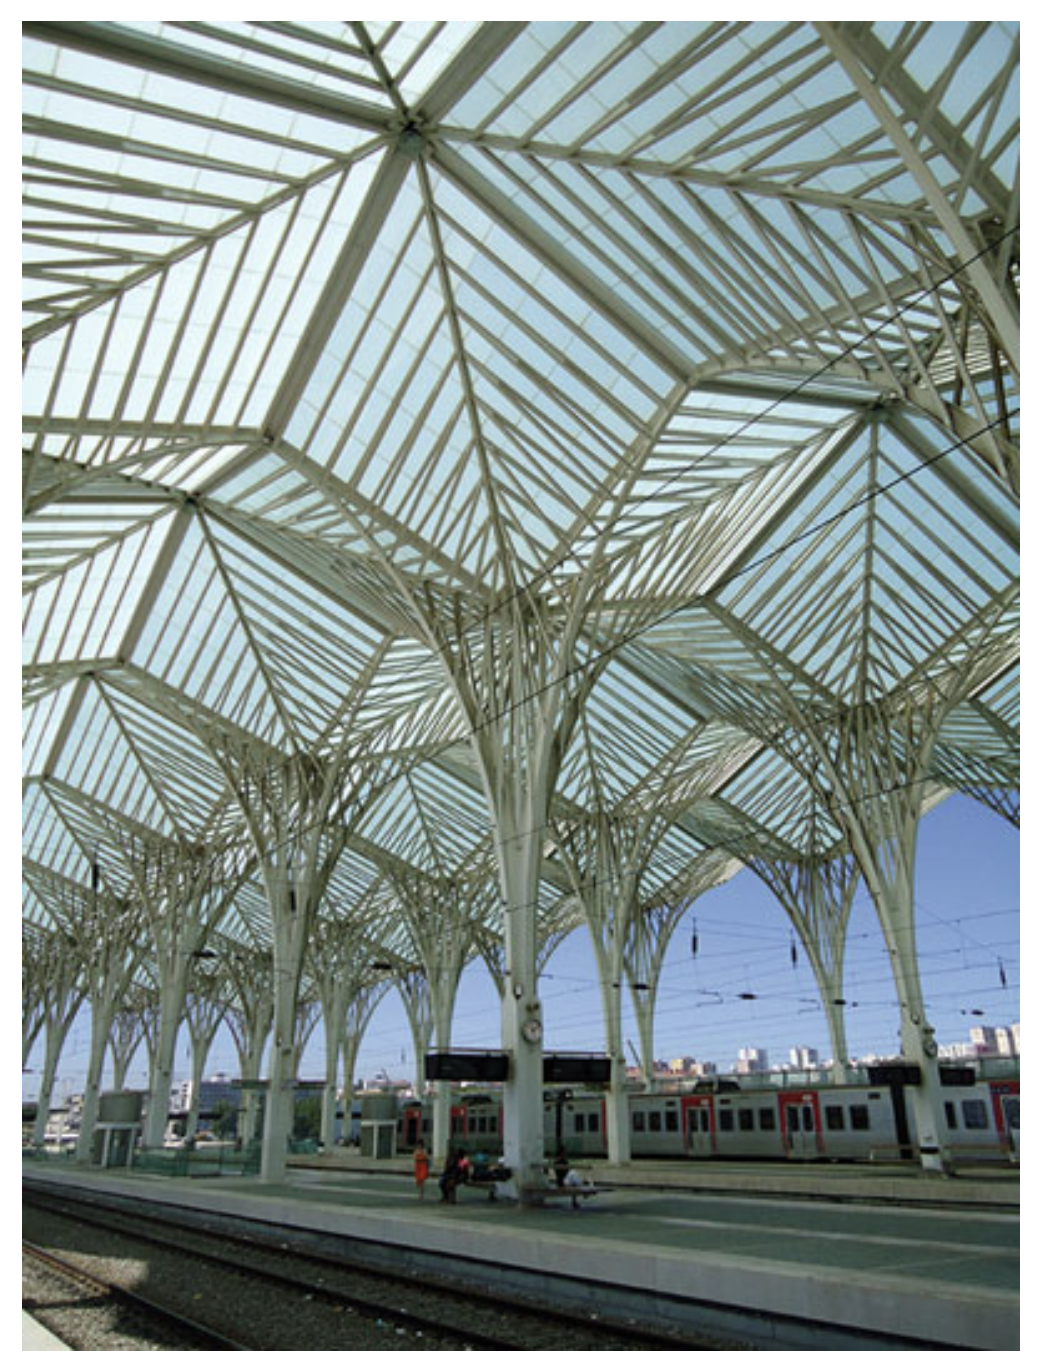
\includegraphics[width=4cm]{../images/beam3d.png}
      \newline\emph{Credit: [N]}
    \end{column}

    \begin{column}{0.65\textwidth}
      \begin{center}
        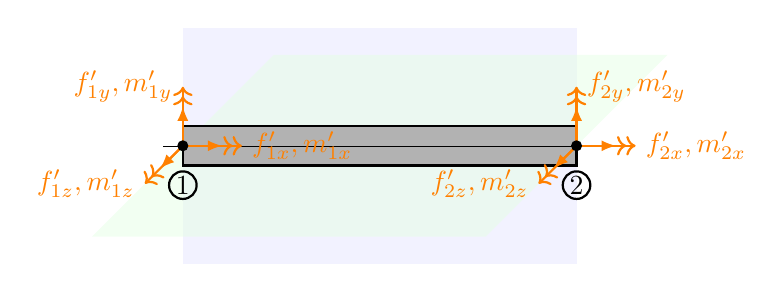
\begin{tikzpicture}[scale=0.5]
          % Oxy plane
          \fill[blue!10, opacity=0.5] (0,-3,0) -- (10,-3,0) -- (10,3,0) -- (0,3,0) -- cycle;

          % Oxz plane
          \fill[green!10, opacity=0.5] (0,0,-6) -- (10,0,-6) -- (10,0,6) -- (0,0,6) -- cycle;

          % Draw the rectangle
          \filldraw[fill=gray!60, draw=black,thick] (0,-0.5) rectangle (10,0.5);
          %axis
          \draw[ultra thin] (-0.5,0) -- (10,0);
          %forces
          \draw[thick,-latex,orange] (0,0) -- (0,1);
          \draw[thick,->>,orange] (0,0) -- (0,1.5) node[left]{$f_{1y}^\prime, m_{1y}^\prime$};
          \draw[thick,-latex,orange] (10,0) -- (10,1);
          \draw[thick,->>,orange] (10,0) -- (10,1.5) node[right]{$f_{2y}^\prime, m_{2y}^\prime$};
          \draw[thick,-latex,orange] (0,0) -- (1,0);
          \draw[thick,->>,orange] (0,0) -- (1.5,0) node[right]{$f_{1x}^\prime, m_{1x}^\prime$};
          \draw[thick,-latex,orange] (10,0) -- (11,0);
          \draw[thick,->>,orange] (10,0) -- (11.5,0) node[right]{$f_{2x}^\prime, m_{2x}^\prime$};
          % moments  
          \draw[thick,-latex,orange] (0,0) -- (0,0,1.5);
          \draw[thick,->>,orange] (0,0) -- (0,0,2.5) node[left]{$f_{1z}^\prime,m_{1z}^\prime$};
          \draw[thick,-latex,orange] (10,0) -- (10,0,1.5);
          \draw[thick,->>,orange] (10,0) -- (10,0,2.5) node[left]{$f_{2z}^\prime,m_{2z}^\prime$};
          % Mark points
          \fill (0,0) circle (4pt);
          \fill (10,0) circle (4pt);
          \draw[thick] (0,0) ++ (0,-1) circle(0.35cm) node {1};
          \draw[thick] (10,0) ++ (0,-1)  circle(0.35cm) node {2};
        \end{tikzpicture}
      \end{center}
      Three-dimensional thin beams are uniaxial (slender) element that can support:
      \begin{itemize}
        \item axial loads $f_{ix}^\prime$,
        \item torsional loads $m_{ix}^\prime$,
        \item bending in the $x^\prime-y^\prime$ plane: $f_{iy}^\prime$ and $m_{iz}^\prime$,
        \item bending in the $x^\prime-z^\prime$ plane: $f_{iz}^\prime$ and $m_{iy}^\prime$.
      \end{itemize}
    \end{column}
  \end{columns}
\end{frame}

{\setbeamercolor{background canvas}{bg=darkred}
\setbeamercolor{block body}{bg=darkred,fg=white}
\setbeamercolor{itemize item}{fg=white}
\setbeamercolor{itemize/enumerate body}{fg=white}
\color{white}
\begin{frame}{Differential equations governing the dynamics of thin 3d beams}
  \begin{center}
    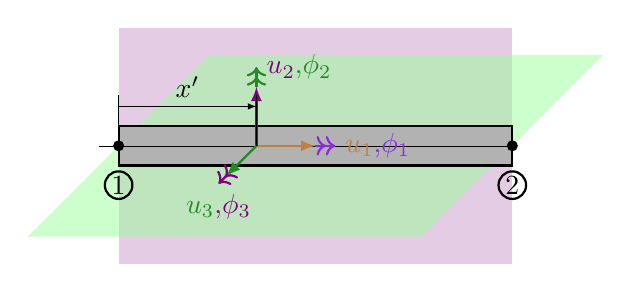
\begin{tikzpicture}[scale=0.5]
      % Oxy plane
      \fill[Purple!40, opacity=0.5] (0,-3,0) -- (10,-3,0) -- (10,3,0) -- (0,3,0) -- cycle;
      % Oxz plane
      \fill[green!40, opacity=0.5] (0,0,-6) -- (10,0,-6) -- (10,0,6) -- (0,0,6) -- cycle;
      % Draw the rectangle
      \filldraw[fill=gray!60, draw=black,thick] (0,-0.5) rectangle (10,0.5);
      %axis
      \draw[ultra thin] (-0.5,0) -- (10,0);
      % displacement
      \draw[thick,-latex,brown] (3.5,0) -- (5,0);
      \draw[thick,-latex,Purple] (3.5,0) -- (3.5,1.5);
      \draw[thick,-latex,ForestGreen] (3.5,0) -- (3.5,0,2);
      \draw[thick,->>,BlueViolet] (5,0) -- (5.5,0) node[right] {{\color{brown}$u_1$},{\color{BlueViolet}$\phi_1$}};
      \draw[thick,->>,ForestGreen] (3.5,1.5) -- (3.5,2) node[right] {{\color{Purple}$u_2$},{\color{ForestGreen}$\phi_2$}};
      \draw[thick,->>,Purple] (3.5,0,2) -- (3.5,0,2.5) node[below] {{\color{ForestGreen}$u_3$},{\color{Purple}$\phi_3$}};
      % length
      \draw[ultra thin] (3.5,0) -- (3.5, 1.3) ;
      \draw[ultra thin] (0,0) -- (0, 1.3) ;
      \draw[-latex, ultra thin]  (0,1)  to node[sloped,midway,above] {$x^\prime$}(3.5,1);
      % Mark points
      \fill (0,0) circle (4pt);
      \fill (10,0) circle (4pt);
      \draw[thick] (0,0) ++ (0,-1) circle(0.35cm) node {1};
      \draw[thick] (10,0) ++ (0,-1)  circle(0.35cm) node {2};
    \end{tikzpicture}
  \end{center}
  \vspace{-0.5cm}
  \begin{tcolorbox}[colback=darkred!10,colframe=darkred!40!black]
    \vspace{-0.5cm}
    \begin{align*}
            & {\color{brown} EA \partial^{2}_{x^\prime x^\prime}u_1(x^\prime, t) = \rho A \ddot{u}_1(x^\prime, t) }
      \quad & {\color{Purple} \partial_{x^\prime x^\prime}^2\big(EI_z\partial_{x^\prime x^\prime}^2u_{2}(x^\prime,t)\big)+\rho A\ddot u_{2}(x^\prime,t)=0 }     \\
            & {\color{BlueViolet} GJ \partial^{2}_{x^\prime x^\prime}\phi_{1}(x^\prime, t) = \rho J \ddot{\phi}_1(x^\prime, t) }
            & {\color{ForestGreen} \partial_{x^\prime x^\prime}^2\big(EI_y\partial_{x^\prime x^\prime}^2u_{3}(x^\prime,t)\big)+\rho A\ddot u_{3}(x^\prime,t)=0}
    \end{align*}
  \end{tcolorbox}
  {\small
  \begin{multicols}{2}
    \begin{itemize}
      \item $E$ Young's modulus of the material.
      \item $A$ cross-sectional area.
      \item $\rho$ material density.
      \item $I_y$ and $I_z$ are the second moments of inertia with respect to $Oy$ and $Oz$.
      \item $J$ polar moment of inertia of the cross-section.
    \end{itemize}
  \end{multicols}
  }
\end{frame}
}

\begin{frame}{Displacements discretization}
  Total of \textbf{six nodal generalized displacements at each unconstrained joint}:
  \begin{itemize}
    \item three translation components $q_{ix}^\prime$, $q_{iy}^\prime$ and $q_{iz}^\prime$ along the $x$, $y$ and $z$ axes,
    \item three rotational components $\phi_{ix}^\prime$, $\phi_{iy}^\prime$ and $\phi_{iz}^\prime$ about the $x$, $y$ and $z$ axes.
  \end{itemize}\vspace{0.2cm}
  $$u^h(x^\prime,t)=  \mathbf H(x^\prime)\mathbf q_{loc} (t)$$

  \begin{columns}
    \begin{column}{0.4\textwidth}
      $$\tiny \mathbf q_{loc} (t)=\begin{bmatrix}
          {\color{brown} q_{1x}^\prime(t)}             \\[2pt]
          {\color{Purple} q_{1y}^\prime(t)}            \\[2pt]
          {\color{ForestGreen} q_{1z}^\prime(t)}       \\[2pt]
          {\color{BlueViolet} \phi_{1x}^\prime(t)}     \\[2pt]
          {\color{ForestGreen} \phi_{1y}^\prime(t)   } \\[2pt]
          {\color{Purple} \phi_{1z}^\prime(t)}         \\[2pt]
          {\color{brown} q_{2x}^\prime(t)}             \\[2pt]
          {\color{Purple} q_{2y}^\prime(t)}            \\[2pt]
          {\color{ForestGreen} q_{2z}^\prime(t)}       \\[2pt]
          {\color{BlueViolet} \phi_{2x}^\prime(t)}     \\[2pt]
          {\color{ForestGreen} \phi_{2y}^\prime(t)   } \\[2pt]
          {\color{Purple} \phi_{2z}^\prime(t)}         \\[2pt]
        \end{bmatrix}$$
    \end{column}

    \begin{column}{0.3\textwidth}
      \tiny  \begin{align*}
        h_1(x^\prime) & = 1-x^\prime/\ell                        \\
        h_2(x^\prime) & =2(x^\prime/\ell)^3-3(x^\prime/\ell)^2+1 \\
        h_3(x^\prime) & =2(x^\prime/\ell)^3-3(x^\prime/\ell)^2+1 \\
        h_4(x^\prime) & = 1-x^\prime/\ell                        \\
        h_5(x^\prime) & =x^\prime(1-x^\prime/\ell)^2             \\
        h_6(x^\prime) & =x^\prime(1-x^\prime/\ell)^2
      \end{align*}
    \end{column}

    \begin{column}{0.3\textwidth}
      \tiny  \begin{align*}
        h_7(x^\prime)    & = x^\prime/\ell                           \\
        h_8(x^\prime)    & =3(x^\prime/\ell)^2-2(x^\prime/\ell)^3    \\
        h_9(x^\prime)    & =3(x^\prime/\ell)^2-2(x^\prime/\ell)^3    \\
        h_{10}(x^\prime) & = x^\prime/\ell                           \\
        h_{11}(x^\prime) & =x^\prime(x^\prime/\ell)(x^\prime/\ell-1) \\
        h_{12}(x^\prime) & =x^\prime(x^\prime/\ell)(x^\prime/\ell-1)
      \end{align*}
    \end{column}
  \end{columns}
\end{frame}

\begin{frame}{Element stiffness matrix in local coordinates}
  The stiffness matrix for a three-dimensional uniform beam element is written as the superposition of the \textbf{axial stiffness} matrix, the \textbf{torsional stiffness} matrix and the \textbf{flexural stiffness} matrix:
  \[\tiny \mathbf K_{loc}=\left[
      \begin{array}{cccccccccccc}
        \frac{EA}{\ell} & 0                     & 0                     & 0               & 0                     & 0                    & -\frac{EA}{\ell} & 0                      & 0                      & 0                & 0                     & 0                     \\[2pt]
                        & \frac{12EI_z}{\ell^3} & 0                     & 0               & 0                     & \frac{6EI_z}{\ell^2} & 0                & -\frac{12EI_z}{\ell^3} & 0                      & 0                & 0                     & \frac{6EI_z}{\ell^2}  \\
                        &                       & \frac{12EI_y}{\ell^3} & 0               & -\frac{6EI_y}{\ell^2} & 0                    & 0                & 0                      & -\frac{12EI_y}{\ell^3} & 0                & -\frac{6EI_y}{\ell^2} & 0                     \\
                        &                       &                       & \frac{GJ}{\ell} & 0                     & 0                    & 0                & 0                      & 0                      & -\frac{GJ}{\ell} & 0                     & 0                     \\
                        &                       &                       &                 & \frac{4EI_y}{\ell}    & 0                    & 0                & 0                      & \frac{6EI_y}{\ell^2}   & 0                & \frac{2EI_y}{\ell}    & 0                     \\
                        &                       &                       &                 &                       & \frac{4EI_z}{\ell}   & 0                & -\frac{6EI_z}{\ell^2}  & 0                      & 0                & 0                     & \frac{2EI_z}{\ell}    \\
                        &                       &                       &                 &                       &                      & \frac{EA}{\ell}  & 0                      & 0                      & 0                & 0                     & 0                     \\
                        &                       &                       &                 &                       &                      &                  & -\frac{12EI_z}{\ell^3} & 0                      & 0                & 0                     & -\frac{6EI_z}{\ell^2} \\
                        &                       &                       &                 &                       &                      &                  &                        & \frac{12EI_y}{\ell^3}  & 0                & \frac{6EI_y}{\ell^2}  & 0                     \\
                        &                       &                       &                 &                       &                      &                  &                        &                        & \frac{GJ}{\ell}  & 0                     & 0                     \\
                        &                       &                       &                 &                       &                      &                  &                        &                        &                  & \frac{4EI_y}{\ell}    & 0                     \\
        sym.            &                       &                       &                 &                       &                      &                  &                        &                        &                  &                       & \frac{4EI_z}{\ell}
      \end{array}
      \right]
  \]
\end{frame}

\begin{frame}{Element consistent mass matrix in local coordinates}
  The consistent mass matrix for a three-dimensional uniform beam element is written as the superposition of the \textbf{axial mass} matrix, the \textbf{torsional mass} matrix and the \textbf{flexural mass} matrix:
  $$\small \mathbf M_{loc}=\frac{\rho A \ell}{420}\left[
      \begin{array}{cccccccccccc}
        140  & 0   & 0   & 0              & 0       & 0       & 70  & 0      & 0       & 0              & 0        & 0        \\
             & 156 & 0   & 0              & 0       & 22\ell  & 0   & 54     & 0       & 0              & 0        & -13\ell  \\
             &     & 156 & 0              & -22\ell & 0       & 0   & 0      & 54      & 0              & 13\ell   & 0        \\
             &     &     & \frac{140J}{A} & 0       & 0       & 0   & 0      & 0       & \frac{70J}{A}  & 0        & 0        \\
             &     &     &                & 4\ell^2 & 0       & 0   & 0      & -13\ell & 0              & -3\ell^2 & 0        \\
             &     &     &                &         & 4\ell^2 & 0   & 13\ell & 0       & 0              & 0        & -3\ell^2 \\
             &     &     &                &         &         & 140 & 0      & 0       & 0              & 0        & 0        \\
             &     &     &                &         &         &     & 156    & 0       & 0              & 0        & -22\ell  \\
             &     &     &                &         &         &     &        & 156     & 0              & 22\ell   & 0        \\
             &     &     &                &         &         &     &        &         & \frac{140J}{A} & 0        & 0        \\
             &     &     &                &         &         &     &        &         &                & 4\ell^2  & 0        \\
        sym. &     &     &                &         &         &     &        &         &                &          & 4\ell^2  \\
      \end{array}
      \right]$$
\end{frame}

\begin{frame}{Transformation of coordinates}
  \begin{itemize}
    \item The stiffness and mass matrices are defined in the local coordinate system $x^\prime$, $y^\prime$ and $z^\prime$ fixed to the beam segment.
    \item To assemble the global stiffness and mass matrices, these local matrices must be transformed into the global coordinate system $x$, $y$, $z$.
  \end{itemize}
  \begin{center}
    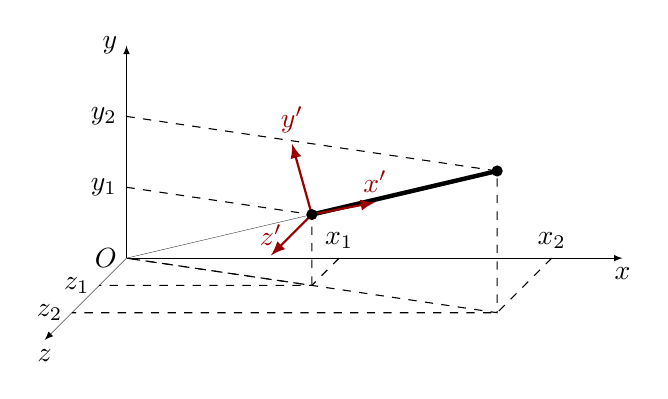
\begin{tikzpicture}[scale=0.9]
      % Draw background grid
      %\draw[step=1cm,gray,very thin] (0,0) grid (12,6);
      % Define coordinates
      \coordinate (A) at (0,0);
      \coordinate (B) at (3,1,1);
      \coordinate (C) at (6,2,2);
      \node[left] at (A) {$O$};
      % Draw the truss members
      \draw[ultra thin] (A) -- (B);
      \draw[ultra thick] (B) -- (C);
      % Global coordinate system
      \draw[-latex, ultra thin] (0,0) -- (0,3) node[left] {$y$};
      \draw[-latex, ultra thin] (0,0) -- (7,0) node[below] {$x$};
      \draw[-latex, ultra thin] (0,0) -- (0,0,3) node[below] {$z$};
      % Local primed coordinate system
      \draw[-latex,thick, darkred] (B) -- ++(1,0.28,0.28) node[above] {$x^\prime$};
      \draw[-latex,thick, darkred] (B) -- ++(-0.28,1,0) node[above] {$y^\prime$};
      \draw[-latex,thick, darkred] (B) -- ++(0,0,1.5) node[above] {$z^\prime$};
      % Draw supports (circles at joints)
      \filldraw (B) circle (2pt);
      \filldraw (C) circle (2pt);
      % draw the projections and the angles
      \draw[thin, dashed] (0,1,0) node[left]{$y_1$}-- (B) -- (3,0,1) -- (A);
      \draw[thin, dashed] (3,0) node[above]{$x_1$} -- (3,0,1) -- (0,0,1) node[left]{$z_1$};
      \draw[thin, dashed] (0,2,0) node[left]{$y_2$}-- (C) -- (6,0,2) -- (A);
      \draw[thin, dashed] (6,0) node[above]{$x_2$} -- (6,0,2) -- (0,0,2) node[left]{$z_2$};
    \end{tikzpicture}
  \end{center}
\end{frame}

\begin{frame}{Direction cosines}
  \begin{itemize}
    \item The relationship between local and global coordinates is:
          $$ \left[
              \begin{array}{c}
                x^\prime \\
                y^\prime \\
                z^\prime
              \end{array}
              \right]
            =\underbrace{ \left[
                \begin{array}{ccc}
                  \cos(x^\prime x) & \cos (x^\prime y) & \cos (x^\prime z) \\
                  \cos(y^\prime x) & \cos (y^\prime y) & \cos (y^\prime z) \\
                  \cos(z^\prime x) & \cos (z^\prime y) & \cos (z^\prime z)
                \end{array}
                \right]}_\text{$\mathbf {T^\prime}$}
            \left[
              \begin{array}{c}
                x \\
                y \\
                z
              \end{array}
              \right]$$
    \item The local $x^\prime$ is given by:
          $$Ox^\prime=\left[l_x,l_y,l_z \right]$$
          where
          $$l_x=\cos(x^\prime x)=\frac{x_2-x_1}{{}^e\ell},\quad l_y=\cos (x^\prime y)=\frac{y_2-y_1}{{}^e\ell},\quad l_z=\cos (x^\prime z)=\frac{z_2-z_1}{{}^e\ell},$$
          $$^e\ell=\sqrt{(x_2-x_1)^2+(y_2-y_1)^2+(z_2-z_1)^2}.$$
  \end{itemize}
\end{frame}

\begin{frame}{Direction cosines}
  \begin{itemize}
    \item The local $y^\prime$ axis is chosen so that it lies in the local $x^\prime-y^\prime$ plane and it is perpendicular to $x^\prime$:
          $$Oy^\prime=\frac{1}{d}\left[l_y,l_x,0 \right]$$
          thus
          $$\cos(y^\prime x)=\frac{l_y}{d},\quad \cos (y^\prime y)=\frac{l_x}{d},\quad \cos (y^\prime z)=0,\quad d=\sqrt{l_x^2+l_y^2}.$$
    \item The local $z^\prime$ axis is chosen so that $Oz^\prime= Ox^\prime\times Oy^\prime$:
          $$Oz^\prime=\frac{1}{d}\left[-l_xl_z,-l_yl_z,0 \right]$$
          thus
          $$\cos(z^\prime x)=-\frac{l_xl_z}{d},\quad \cos (z^\prime y)=-\frac{l_yl_z}{d},\quad \cos (z^\prime z)=d.$$
  \end{itemize}
\end{frame}

\begin{frame}{Global displacements for oriented three-dimensional beam}
  \vspace{-0.5cm}

  \begin{columns}
    \column{0.5\textwidth}
    \small $$\underbrace{ \begin{bmatrix}
          {\color{black} q_{1x}^\prime(t)}       \\[2pt]
          {\color{black} q_{1y}^\prime(t)}       \\[2pt]
          {\color{black} q_{1z}^\prime(t)}       \\[2pt]
          {\color{black} \phi_{1x}^\prime(t)}    \\[2pt]
          {\color{black} \phi_{1y}^\prime(t)   } \\[2pt]
          {\color{black} \phi_{1z}^\prime(t)}    \\[2pt]
          {\color{black} q_{2x}^\prime(t)}       \\[2pt]
          {\color{black} q_{2y}^\prime(t)}       \\[2pt]
          {\color{black} q_{2z}^\prime(t)}       \\[2pt]
          {\color{black} \phi_{2x}^\prime(t)}    \\[2pt]
          {\color{black} \phi_{2y}^\prime(t)   } \\[2pt]
          {\color{black} \phi_{2z}^\prime(t)}    \\[2pt]
        \end{bmatrix}}_\text{$\mathbf q_{loc} (t)$} = \underbrace{ \begin{bmatrix}
          \mathbf {T^\prime} &                    &                    &                    & \\
                             & \mathbf {T^\prime} &                    &                      \\
                             &                    & \mathbf {T^\prime} &                      \\
                             &                    &                    & \mathbf {T^\prime}   \\
        \end{bmatrix}}_\text{$\mathbf T$} \underbrace{ \begin{bmatrix}
          {\color{black} q_{1x}(t)}       \\[2pt]
          {\color{black} q_{1y}(t)}       \\[2pt]
          {\color{black} q_{1z}(t)}       \\[2pt]
          {\color{black} \phi_{1x}(t)}    \\[2pt]
          {\color{black} \phi_{1y}(t)   } \\[2pt]
          {\color{black} \phi_{1z}(t)}    \\[2pt]
          {\color{black} q_{2x}(t)}       \\[2pt]
          {\color{black} q_{2y}(t)}       \\[2pt]
          {\color{black} q_{2z}(t)}       \\[2pt]
          {\color{black} \phi_{2x}(t)}    \\[2pt]
          {\color{black} \phi_{2y}(t)   } \\[2pt]
          {\color{black} \phi_{2z}(t)}    \\[2pt]
        \end{bmatrix}}_\text{$\mathbf q(t)$}$$

    \column{0.55\textwidth}
    \begin{center}
      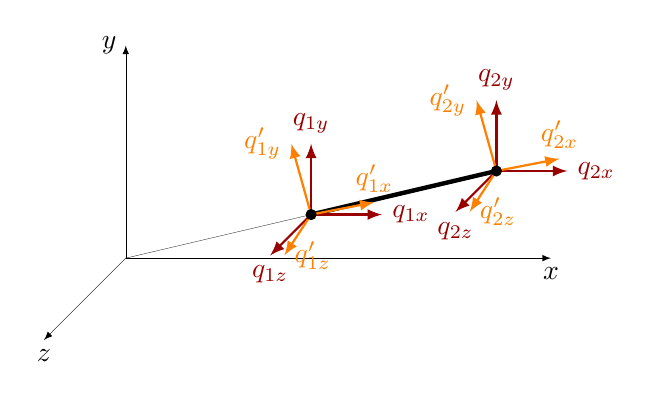
\begin{tikzpicture}[scale=0.9]
        % Draw background grid
        %\draw[step=1cm,gray,very thin] (0,0) grid (12,6);
        % Define coordinates
        \coordinate (A) at (0,0);
        \coordinate (B) at (3,1,1);
        \coordinate (C) at (6,2,2);
        % Draw the truss members
        \draw[ultra thin] (A) -- (B);
        \draw[ultra thick] (B) -- (C);
        % Global coordinate system
        \draw[-latex, ultra thin] (0,0) -- (0,3) node[left] {$y$};
        \draw[-latex, ultra thin] (0,0) -- (6,0) node[below] {$x$};
        \draw[-latex, ultra thin] (0,0) -- (0,0,3) node[below] {$z$};
        % Local coordinate systems
        \draw[-latex, darkred, thick] (B) -- ++(0,1) node[above] {$q_{1y}$};
        \draw[-latex, darkred, thick] (B) -- ++(1,0) node[right] {$q_{1x}$};
        \draw[-latex, darkred, thick] (B) -- ++(0,0,1.5) node[below] {$q_{1z}$};
        \draw[-latex, darkred, thick] (C) -- ++(0,1) node[above] {$q_{2y}$};
        \draw[-latex, darkred, thick] (C) -- ++(1,0) node[right] {$q_{2x}$};
        \draw[-latex, darkred, thick] (C) -- ++(0,0,1.5) node[below] {$q_{2z}$};
        % Local 
        \draw[-latex,thick, orange] (B) -- ++(1,0.28,0.28) node[above] {$q_{1x}^\prime$};
        \draw[-latex,thick, orange] (B) -- ++(-0.28,1,0) node[left] {$q_{1y}^\prime$};
        \draw[-latex,thick, orange] (B) -- ++(0.2,0,1.5) node[right] {$q_{1z}^\prime$};
        \draw[-latex,thick, orange] (C) -- ++(1,0.28,0.28) node[above] {$q_{2x}^\prime$};
        \draw[-latex,thick, orange] (C) -- ++(-0.28,1,0) node[left] {$q_{2y}^\prime$};
        \draw[-latex,thick, orange] (C) -- ++(0.2,0,1.5) node[right] {$q_{2z}^\prime$};
        % Draw supports (circles at joints)
        \filldraw (B) circle (2pt);
        \filldraw (C) circle (2pt);
      \end{tikzpicture}
    \end{center}
  \end{columns}
\end{frame}

\end{document}